\section{Implementation}
%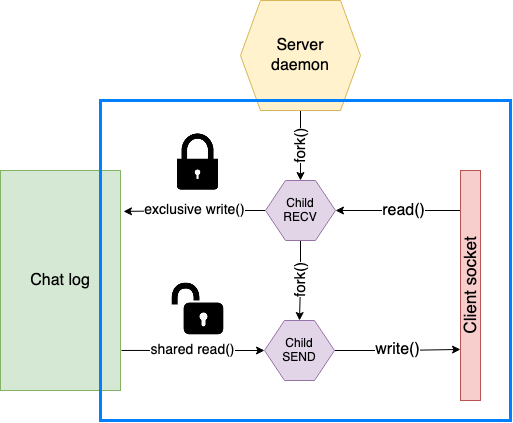
\includegraphics[width=1in,height=1.25in,keepaspectratio]{img/server.png}
\begin{figure}[!t]
	\centering
	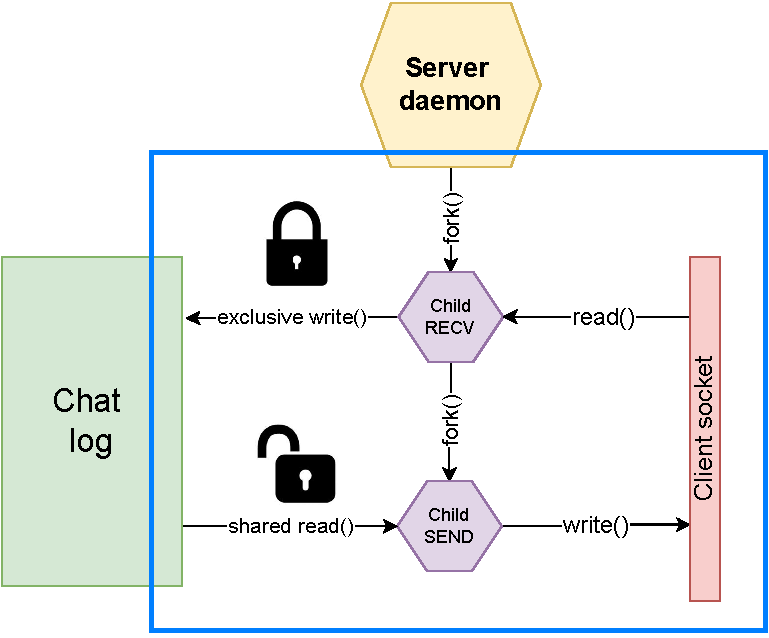
\includegraphics[width=2.5in]{img/server.pdf}
	%where an .eps filename suffix will be assumed under latex, 
	%and a .pdf suffix will be assumed for pdflatex; or what has been declared
	%via \DeclareGraphicsExtensions.
	\caption{Server's back-end architectural overview. The blue rectangle denotes the process cluster created exclusively for each client taking part in a chat service.}
	\label{fig_server_backend}
\end{figure}
The requirements for the chat application are that an undefined number of participants can simultaneously exchange text messages in a chatroom. Furthermore, the communication might be asynchronous, so that the participants can read messages sent to them while they were not connected to the server. The application should use the least amount of dependencies as possible to enable portability across Unix systems, i.e. the chat server should compile natively with the same source file in FreeBSD or in a Linux distribution.

The server fundamentally requires a process working as a daemon accepting incoming connection attempts from clients. For each accepted client connection there are multiple possibilities regarding the architecture of the server. The daemon could handle each client separately in a unique thread or child process.

The server will mostly have an IO-bound workload, consisting of handling asynchronous network packets and writing the messages from the users into files in the server's filesystem. An IO-bound workload benefits from the use of a pre-emptive scheduler, since the threads or processes are constantly changing alternatively between a blocked and an unblocked state in an unpredictable manner. As soon as a client goes silent the pre-emptive scheduler can run any other runnable process \cite{Kennedy2018}. Hence, the context-switching is actually advantageous for IO-bound workloads, whereas in CPU-bound workloads (e.g. intensive long-running sequential computations) it becomes a performance bottleneck.

Therefore, handling each client connection separately by forking a child process seems like a good fit for the kind of workload that is expected. Nonetheless, it must be acknowledged that a counterargument against using processes is that thread creation and context-switching times in threads are generally faster than for processes, since processes have an inherently more complex memory layout than threads \cite{Kerrisk2010}.

However, other reasons settled the decision towards processes instead of threads. Before going into these reasons, it makes sense to review the architecture that was actually implemented as a solution. Figure \ref{fig_server_backend} shows a high-level representation of how the server handles every client connection. After successfully authenticating a client, the server daemon calls the \textit{fork} syscall and creates a new child process exclusively for the new client.
 
This child process, called "\textit{Child RECV}" in fig. \ref{fig_server_backend}, inherits a copy of the newly established socket which handles the client. Child RECV is responsible for reading any incoming messages from the client, writing these messages in a concurrently-safe way into a central chat log, sending a multicast signal to let all other clients know that there is a new message and creating a further child process called "\textit{Child SEND}". \textit{Child SEND} also inherits the client's socket in order to send the messages stored in the central chat log at an appropriate time to the client. The blue rectangle depicted in figure \ref{fig_server_backend} comprises a single process cluster for a particular client. For every client connected simultaneously to the server there is one of this process clusters running concurrently.

 Compartmentalizing the different clients into separate processes has the intrinsic advantage of granting more availability in case of a distributed denial of service (DDoS) attack or simply heavy traffic in the server's public-facing daemon. If for any reason, the daemon is getting cluttered with connection attempts, to a point in which the high load threatens to affect the communication performance of the clients already participating inside a chat service, then the daemon's process can be temporarily stopped, or even killed, so that the public-facing port is closed. Since each client's process cluster works completely independently from the daemon accepting new clients and from all other clients' process clusters, the service can continue uninterrupted for all clients already connected. 
 
 From a system administration perspective it is also very convenient to handle each client connection with different processes, since it makes the monitoring and administration of system resource utilization in a \textit{per-client} granular way easy through the use of command line tools like \textit{kill}, \textit{ps}, \textit{ss} or \textit{sockstat}, and \textit{top}.

\subsection{Transactional isolation and atomicity}
Although the data model of the chat application would fit well within a relational database, since the types of the data fields for every message exchange are immutable and translatable into the data types used in relational databases, the system intentionally avoids using any kind of external database system. This design decision makes the application more easily portable and deployable, due to the fact that the same executable of the chat server entirely handles the message storing and retrieving for all data exchanges. Deploying the chat server into a cloud server is as easy as pulling the repository, compiling and running the binary, there is no need to first install and configure a (No)SQL server.

Nonetheless, this implies that the chat program has to fulfil some data safety guarantees that would otherwise be outsourced entirely to the database management system (DBMS). Mainstream DBMS have the ability to perform a series of reads and writes to the underlying data system as a single "\textit{logical unit}" \cite{Kleppmann2017}, a so-called "\textit{transaction}". A transaction is useful as a way of ensuring atomicity and isolation within a distributed system.

Since the incoming messages from the clients will all be centrally stored in a log file and messages from different clients can arrive at any time simultaneously to the server, a transactional mechanism is implemented to avoid race conditions. 

Therefore, the data management system must fulfil the following four requirements. Multiple clients simultaneously writing to the log file should not over-write their messages. Furthermore, it should not be possible to read the log file during a write-operation from another client to avoid reading incomplete data, and, conversely, it should not be possible to write to the log, while another client is reading from it. Finally, unlimited concurrent reading operations from multiple clients are permitted on the log file, since reading from the log file does not have any side effects on the stored data.

To satisfy these criteria, the server creates and opens the central log file with the "\textit{O\_APPEND}" flag (append mode), so that before each write to the file the offset is positioned at the end of the file and the write operation is subsequently performed in a single atomic operation \cite{Kerrisk2010}. Thus, old data written to the log cannot get corrupted by new writes to the file.

Moreover, a file locking system is implemented using the \textit{flock} syscall, in order to fulfil the previously mentioned four requirements. Two different types of locks can be placed on a file: a shared lock and an exclusive lock. When multiple clients try to simultaneously send messages to the chat log, the child process Child RECV tries to place an exclusive lock on the chat log file.  If no other lock is currently placed on the file, Child RECV can write exclusively into the chat log until the placed lock is released. Meanwhile, no other process can write or read from the file, the other Child RECV processes trying to write to the chat log file would block on the call to flock, until the process holding the exclusive lock releases it. All the necessary writes to the chat log file would be scheduled sequentially.

Conversely, when the server sends new messages to a client through Child SEND, it has to read the messages from the chat log. Hence, the child process places a shared lock on the chat log and reads from it. Any other process trying to simultaneously read from the same file can place another shared lock and read from the file, but a process trying to write to the file would block when placing the exclusive lock, until all shared locks have been released. 

This file handling architecture makes sending messages to multiple clients a highly parallelizable operation, while writing to the chat log is a secure isolated task performed in an atomic way.

\subsection{Multicasting with Unix IPC}
The system should deliver new messages instantly through the respective Child SEND process of every client each time a new message is received, in other words, every message must be multicasted to all participating clients. The number of connected clients can change over time and it is unlimited. 

The two main IPC (inter-process communication) mechanisms capable of multicasting to multiple processes are sockets and POSIX signals \cite{Kerrisk2010}. Signals are used in this implementation, because from a software engineering perspective configuring sockets to handle multicasting is less portable and requires more code-refactoring.

The Unix standard \textit{SIGUSR1} signal, which is reserved for "user defined behaviour", can be used to synchronously inform a group of processes about an event, in this case, the need to send new messages to the clients.

By choosing to multicast with signals the possibility to work with threads, instead of with processes, is eliminated. Since all threads in a process share the same signal dispositions and for this design a different signal disposition between parent and child processes is a requirement. Moreover, this architecture does not require a centralized administrative process constantly monitoring which clients are currently online, to whom the messages should be delivered. Instead, it outsources this task to the kernel which manages signal distribution.


\subsection{Portability issues}
Even though, only portable Unix syscalls are used and the number of dependencies is reduced to the utmost minimum of GCC and the C standard library, some portability issues arise when deploying in a multi-platform fashion.

The back-end was compiled with GCC and tested in two different Debian-based distros: Ubuntu and Kali Linux, the former was a 32-bit system. A single compilation difference between the two platforms rendered the back-end service completely useless in one instance. The root cause of the faulty behaviour was then established using a syscall and signals monitoring tool like \textit{strace} in a very cumbersome process. The bug was caused by a difference in the default flags assigned by the compiler to the syscall assigning a signal disposition.

Thus, it is illusory to think that restricting the dependencies to the bare minimum of the C standard library and GCC will make the code perfectly compatible across GNU/Linux systems. Debugging unexplained behaviour will still be arduous.

\subsection{Security}
The chat server runs as a long-lasting daemon, therefore leaving at least one port open to the public internet from which the clients will establish a connection with the server. It must be taken for granted that the open port will eventually be discovered by web-scanning botnets that periodically scan targeted hitlists (specially known IP ranges from cloud providers) or random IP ranges \cite{Mirkovic2004}\cite{Graham}. Accordingly, it is necessary to secure the application to not compromise the infrastructure.

The back-end service is not run inside a container, since this would reduce the portability across Unix systems, e.g. the BSDs do not have kernel features such as cgroups and Linux namespaces, which make natively running typical container management systems like Docker impossible \cite{Kerrisk2021}.

An alternative way of sandboxing the application without containers is running the service as a specially created system user account with the minimum amount possible of privileges. Thereupon, even if the service is compromised the amount of possible damage is limited to the reduced capabilities of the system user. Furthermore, a long authentication token is required to access any given chat session.